

%\documentclass[conference]{IEEEtran}
\documentclass[12pt,a4paper]{article}
\usepackage{fullpage}

\usepackage{graphics}
\usepackage{color}
\usepackage[pdftex]{hyperref}
\usepackage{graphicx}

\begin{document}
%
% paper title
% can use linebreaks \\ within to get better formatting as desired
\title{A Survey of Physical Design Techniques of Information Systems}


% author names and affiliations
% use a multiple column layout for up to three different
% affiliations
%\author{\IEEEauthorblockN{Karim Ali, Sarah Nadi}
%\IEEEauthorblockA{School of Computer Science\\
%University of Waterloo\\
%Email: {{karim, snadi}}@uwaterloo.ca}
%}

\author{Karim Ali and Sarah Nadi\\
\{karim, snadi\}@cs.uwaterloo.ca \\
David R. Cheriton School of Computer Science\\
University of Waterloo\\
}


% make the title area
\maketitle


\begin{abstract}
%\boldmath
The abstract goes here.
\end{abstract}

\section{Introduction}

Database users write queries and updates using a "user-friendly" language such as SQL without having to worry about how the underlying data is stored. Physical database design is concerned with the actual storage of data on disk. This means how the files are organized, and how they are accessed. Data is stored in the form of records in files which reside on a physical disk. In this sense, we try to find the most efficient way possible to store and access the data such that queries are answered and executed efficiently. This is reflected in designing proper indexing techniques, partitioning data for more efficient access, designing materialized views, data clustering, data compression, striping, mirroring and denormalization~\cite{lightstone2007physical}. 

This survey presents the different physical design patterns that have been used in different types of information systems. The systems discussed in this survey are disk based relational databases, main memory relational databases, data warehouses, and XML databases. The aim of this survey is not to explain the details of every data structure used in physical design, but rather to compare how the different data structures have been used in these systems. This includes explaining how alterations or additions are made to data structures to fit the specific needs of every system. For a complete reference on the details of the data structures used in physical database design, please see (CITE HERE). 

The rest of the survey is organized as follows. Section~\ref{SEC-ELEMENTS} first explains different elements of physical database design. For example, this includes explaining what indexes are and briefly mentioning what the different types of indexes used in information systems are. After explaining the different elements of physical database design, Section~\ref{SEC-DIFFSYS} discusses how each of the four systems uses these elements to improve its efficiency. Sections~\ref{SEC-DDRDB},~\ref{SEC-MMDB},~\ref{SEC-WAREHOUSES},~\ref{SEC-XML} discuss Disk Based Databases, Main Memory Databases, Data Warehouses, and XML Databases respectively. Throughout these sections, comparisons are made as to how the different elements have been modified to fit the needs of each system. Section~\ref{SEC-AUTO} then presents physical database design can be automated. Section~\ref{SEC-OPEN} mentions some of the open problems of physical database design, and suggests possible solutions. Finally Section~\ref{SEC-CONCL} summarizes and concludes this summary.


\section{Elements of Physical Database Design}
\label{SEC-ELEMENTS}

\subsection{Indexes}

The first physical database design decision to be considered is the choice of indexes to be implemented. The concept of indices has been around for a long time.
Just like and index at the end of the book is provided to help find certain content faster, indices in an information system help find content in tables faster.
The main idea of an index is to have each record in a table have a unique identifier (primary key) and then organize these identifiers in a certain way that
allows for fast access of a specific record. Of course, indexing can be done on any column in the database and not necessarily the primary key. There are many
type of indexes that have been used in information systems.
B-trees (short for Balanced Trees) are the most used database index structure.  The B-tree is essentially similar to the traditional Binary Search Tree, but
instead of having one value per node, a B-tee can have many values per node~
cite{comer1979ubiquitous} as shown in Figure (PUT A FIGURE FOR A B TREE HERE). B-trees are suitable for relational databases since the cost of retrieval in a B-tree is at most proportional to: $log_{d}\frac{n+1}{2}$. The cost of insertion and deletion is at most proportional to $log_{d}n$ due to the possibility of progressing back up the tree to balance it after an insertion or a deletion. Although B-trees do well in retrieval, deletion and insertion, they do not perform well in sequential search. 

Different variations of B-trees have been used. For example, $B^{+}-trees$ are now the main method of indexing in Disk Based Relational Databases (DRDB). These will be discussed in Section~\ref{SEC-DDRDB}. The T Tree has been proposed for main memory databases, and will be discussed in Section~\ref{SEC-MMDB}. Cache sensitive indexes were then proposed. A variation of T Trees, Cache Sensitive T-Trees (CST-Trees) was introduced, and is also discussed in Section~\ref{SEC-MMDB}. On the same note, Cache Conscious $B^{+}-trees$ and Prefetching $J^{+}-Trees$ are also discussed in Section~\ref{SEC-MMDB}. 

Of course, there are other indexing techniques used such as hash tables, and bitmap indices. For example, Bitmap indices are commonly used in Data Warehouses, and will be discussed in details in Section~\ref{SEC-WAREHOUSES}.

\subsection{Materialized Views}

In a large database system, there are usually a few complex queries that require the joining of many large tables. If these queries are frequently run, then the database performance is likely to suffer, and users have to wait for a long time to get the results back. If we know these queries beforehand, it makes sense to simply store the results of the queries on disk instead of recomputing them each time. This is exactly what materialized views aim to do. By precalculating the results of a complex query, and storing them in a table on disk, the new table with the results is very likely to be much smaller than the original tables decreasing I/O access costs and thus increasing performance~\cite{lightstone2007physical}. Once a materialized view exists, the user can either explicitly query the materialized view, or enter the original query, and have the query optimizer rewrite the query to use the materialized views instead of the original tables. Query rewriting using materialized views is a very popular database research topic (CITE SOME REFERENCES), but is beyond the scope of this survey.

Despite the fact that materialized views provide a significant improvement in performance, we cannot simply create a materialized view for each common query. To begin with, materialized views consume disk storage which might be limited. The second, and main, problem with materialized views is their maintenance. Ensuring that the views have the most up to date data is tricky, and may outset the benefit of using materialized views if it is not properly designed. Finally, having several materialized views may increase the cost of searching for the appropriate view to use during the query optimization stage. Data warehouses heavily rely on materialized views since they have many queries with several joins. This will be discussed in details in Section~\ref{SEC-WAREHOUSES}.

Many query optimization techniques have relied on rewriting queries using views (E.g.~\cite{levy1995answering, gupta1995aggregate, goldstein2001optimizing, abiteboul1998complexity}).

\subsection{Partitioning}

Partitioning is an important aspect of physical design as it reduces table scanning time. There are two main categories of partitioning: horizontal partitioning
and vertical partitioning. Horizontal partitioning divides the table into sets of table rows where each row or record still has all the attributes of the table.
For example, dividing the data by date where all data dating less than year 2000 lies in one partition while all data dating more lies in another. On the other
hand, vertical partitioning reduces the width of the dataset by storing some attributes in one table, and some in another.
The main advantage of any type of partitioning is to reduce the amount of time it takes to scan a table which in turn improves performance. For example, if a
table has 1000 records, and a query is only using the first 20 records then having these 20 records in a partition containing 50 records will save time as
opposed to examining all the 1000 records. Further classification in partitioning is single vs group horizontal or vertical
partitioning~\cite{gruenwald1990database}. Horizontal partitioning just divides the data into partitions where each group contains complete tuples. Group
horizontal partitioning groups tuples that are more frequently used together. Single vertical partitioning divides a relation into groups each of which contains
only one type of attribute. Group vertical partitioning divides the data vertically such that attributes that are commonly required together are physically
stored together.


\subsection{Clustering}
When only records satisfying certain criteria are need from a table, it is often unnecessary to scan the whole table. For example, if only records that occurred
in January 2010 are needed, then querying all the table would be an extremely unnecessary overhead. This is where clustering comes in. Clustering reflects how
the records are physically located together on disk. Records that are likely to be queried together will be stored physically together to avoid querying the
whole table. For the previously mentioned example, the data can be clustered by month, such that all the records of January 2010 are physically in the same
page, for example. In this case, only this page will need to be read. As
people realized the potential of clustering, multidimensional clustering was introduced where data is clustered based on different criteria at the same time.

\subsection{Data Compression}

\subsection{Other Techniques}

Striping, mirroring, denormalization.

\section{Physical Design of Different Information Systems}
\label{SEC-DIFFSYS}

Given the different physical design methods explained in the previous section, we now look at how these methods apply to different types of information systems. Mainly, how they apply to Disk-based relational database systems, main memory relational database systems, data warehouses, and XML databases.

\subsection{Disk Based Relational Database System (DRDB)}
\label{SEC-DDRDB}

Relational Databases were first introduced by Codd~\cite{codd1970relational}
In relational databases, users specify the actions they want to execute without having to worry about how these operations will actually be performed. This is where the role of physical design comes in. Physical design specifies the access paths used to get data from the tables. This includes which indices to use, and in which order to access the tables~\cite{finkelstein1988physical} and so on.


There are many variations of B-trees. In relational databases, the most popular index is the $B^{+}-tree$. The $B^{+}-tree$ is a variant of the B  tree which is becoming the main indexing method supported by many databases such as DB2, Oracle, and SQL Server~cite{lightstone2007physical}. The main difference between the $B^{+}-trees$ and the B-tree is that only leaf nodes contain data pointers in a $B^{+}-tree$. (COMPARE COST HERE). In Prefix $B^{+}-trees$, instead of using the actual key value of a record, a prefix from the key value is used to decrease the storage size needed which will in turn allow more records to be stored per node thus decreasing the height of the tree.

The B+tree is the main indexing method used in current relational databases~\cite{lightstone2007physical}. B+trees have been successful in relational databases since data is ultimately recorded in files. Since B+trees have a high fanout, they allow less I/O operations to access a specific data record which is stored in a specific file.


\subsection{Main Memory Relational Database System (MMDB)}
\label{SEC-MMDB}

A Main Memory Database (MMDB) is one where the data resides in the main memory of the system rather than on a disk~\cite{garcia1992main}. It should be noted that this is different from caching. Disk based database systems use the main memory to cache query results. However, MMDB's primary copy of the data resides in main memory. MMDB have many implementation challenges that have been addressed throughout the research community.

Garcia-Molina and Salem~\cite{garcia1992main} mention some of the challenges involved. One is concurrency control. In disk based databases, locks are tracked through a hash table, but the actual objects on disk do not contain lock information. On the other hand, in MMDB, lock status is part of the object itself since it is cheap to keep a number of bits for that. The next challenge is access methods. In disk-based databases, B-Trees are used to index the data for faster access. B-Trees have a short bushy nature to try to decrease the height of the tree to decrease the number of I/O accesses. Since I/O access is not a problem in MMDB, longer tree structures are used since its cheap to access main memory. Another point is that data values do not need to be stored in the index itself since they will be stored in main memory anyways so there are no performance gains from storing them in the index itself. 

\subsubsection{Type of Indexes Used}

Two considerations are taken when designing index structures for MMDB. The first is that the data resides in main memory and not on disk, and so many of the
considerations taken for I/O operations is no longer there. The second is having index structures cache conscious. Lots of research work has shown that cache
performance is very critical in MMDBs~\cite{rao1999cache, boncz1999database}. This is because the big difference between processor speed and main memory access
speed. Thus, a cache miss is still relatively expensive in main memory databases. Accordingly, we will see that many of the index data structures proposed for
main memory databases focused on being cache conscious or cache sensitive.

cite~\cite{dewitt1984implementation}.

\subsubsection*{$B^{+}-Trees$}
The $B^{+}-Tree$, explained in the previous section, is originally designed for disk based database systems. However, it has also been found useful for main memory databases (REF) as it is cache conscious.


\subsubsection*{T Trees}
Lehmen and Carey~\cite{lehman1986study} study the different features needed for indices of MMDB. When designing data structures for MMDB, we are mainly concerned with the efficient use of CPU cycles and memory. Accordingly, the main goal of an index structure for MMDB is to minimize the overall computation time while using the minimum memory possible. Since all the database data is in main memory, index structures do not need to store actual values like those in disk-oriented databases. Instead, a pointer to the data instead of the actual data can be stored. Lehmen and Carey introduce a new index structure, the T Tree, which combines the features from AVL Trees and B Trees that are suited to main memory. Figure~\ref{fig:ttree} shows the proposed structure of the T Tree. They run some experiments on data residing in main memory to compare the performance of the T Tree to existing structures. All structures were modified to contain pointers to data values rather than the data values themselves. The structures included were  AVL Trees, simple arrays, B Trees, Chained Bucket Hashing, Extendible Hashing, Linear Hashing and Modified Linear Hashing. Their experiments showed that for unordered data, Modified Linear Hashing gave the best performance, and for ordered data, T Trees gave the best performance for a mix of searches, inserts and deletes.


\begin{figure}[!t]
\centering
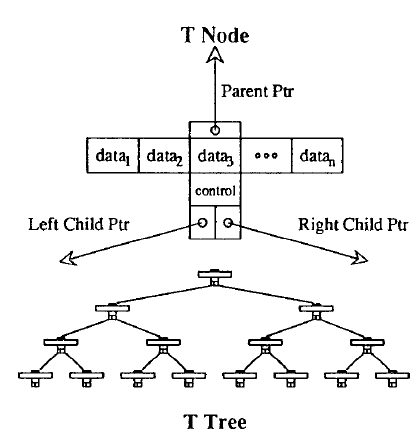
\includegraphics[width=9cm]{figs/Ttree.png}
\caption{T Tree by Lehmen and Carey~\cite{lehman1986study}}
\label{fig:ttree}
\end{figure}

\subsubsection*{Cache Sensitive Search Trees (CSS-Trees)}
\cite{rao1999cache}.


\subsubsection*{Cache Sensitive T-Trees (CST-Trees)}

T Trees were the main index structure used for main memory databases for some time after their proposal. However, it was discovered that B+-trees outperform T-Trees on modern processors because of the growth of cache miss latency relative to processor speed~\cite{rao1999cache,lee2007cst}. This is because the height of the tree is high which makes the total number of memory accesses from the root to the leaf node higher. The other reason is that the node size is not aligned with the cache line size. The other problem with T-Trees is that there is a big waste of space in the cache because unnecessary data is brought into the cache. Additionally, record pointers stored in the tree take up a lot of space.

To resolve these issues, Lee et al.~
cite{lee2007cst} propose the Cache Sensitive T-Trees (CST-Trees). This is achieved in the following ways. First, a binary search tree whose node values are the maximum key of each node in the T Tre is constructed. That way, for a given value, the node containing this value could be quickly located through searching the binary tree. Second, the need to store pointers is eliminated by storing the tree in an array and locating the necessary nodes through index calculation. Finally, node sizes are aligned with cache line size such that there are no cache misses when accessing data in each binary search tree in the array.

\subsubsection*{Cache Sensitive $B^{+}-trees$ ($CSB^{+}-trees)$}

Rao and Ross~\cite{rao1999cache} show that $B^{+}-trees$ are more cache conscious than binary search trees and T-Trees which means they are more suited to main memory databases. However, traditional B+-Trees still had poor cache performance. Therefore, they propose Cache Sensitive B+-Trees ($CSB^{+}-Trees$)~\cite{rao2000making} as an index structure for main memory. To do so, they eliminated most of the child pointers and had more keys in each node to improve locality and reduce tree height~\cite{luan2009prefetching}. Since the number of cache misses in search operations is proportional to the height of the tree, $CSB^{+}-trees$ have fewer cache misses, and thus better performance.

\subsubsection*{$Prefetching B^{+}-Trees (pB^{+}-trees)$}

Chen et al.~\cite{chen2001improving} propose using prefetching to improve the performance of $B^{+}-trees$. Since current computer systems can prefetch different data simultaneously, the author take advantage of this. The node size of the $B^{+}-tree$ is made wider than the cache line size. This way, several cache misses can be overlapped at the same time thus improving performance.

\subsubsection*{$J^{+}-trees$ and $pJ^{+}-trees$}

\subsection{Partitioning}

Partitioning is used in disk based systems to divide the data into the physical pages in a way that will yield the best performance. This could be through
vertical partitioning or horizontal partitioning, as previously explained. In main memory databases, we do not have the issue of expensive disk access which
makes partitioning in memory unnecessary as it will not save any costs. However, partionining is needed in the secondary storage of the data on
disk~\cite{gruenwald1990database}. Disk storage is still used as a backup of main memory databases. When a crash occurs, a reload of the database from disk or
archive memory takes place. In order to avoid page faults caused by referencing data that is still being reloaded, the reloading process must be designed to be
efficient in loading the important data such that the database users are not affected. Gruenwald and Eich~\cite{gruenwald1990database,gruenwald1990choosing}


\subsection{Clustering}
Clustering in disk based systems is important because sequential I/O access is cheaper than random or dispersed I/O access. This is not the case with main
memory, and so clustering is not needed in MMDB~\cite{garcia1992main, moldovan2008databases}. Therefore, components of one object may be spread across memory
without impacting performance.




\subsection{Data Warehouses}
\label{SEC-WAREHOUSES}
A data warehouse is a subject-oriented, integrated, time-variant, and non-volatile collection of data and decision support technologies, aimed at enabling the knowledge worker (executive, manager, analyst) to make better and faster decisions \cite{560407, 248616}. More than half of IT executives named Data warehousing as the highest-priority post-millennium project for them \cite{sen2005comparison}. The value of data warehousing for an organization depends on the organization's need for reliable, consolidated, unique and integrated reporting and analysis of its data, at different levels of aggregation.

Data warehousing has been shown useful in many industries: manufacturing (for order shipment and customer support), retail (for user profiling and inventory management), financial services (for claims analysis, risk analysis, credit card analysis, and fraud detection), transportation (for fleet management), telecommunications (for call analysis and fraud detection), utilities (for power usage analysis), and healthcare (for outcomes analysis) \cite{248616}.

Data warehouses tend to be extremely large, in fact it is quite possible for a data warehouse to store tens of petabytes of data and load tens of terabytes of data everyday \cite{thusoo2010data}. Datta et al. \cite {628286} notes that the information in a data warehouse is usually multidimensional in nature, requiring the capability to view the data from a variety of perspectives. Aggregated and summarized data become more crucial than detailed records in such environment. Therefore, the workloads are query intensive with mostly ad hoc, complex queries, often requiring computationally expensive operations such as scans, joins, and aggregation. Performing such operations on large amounts of data, like in the case of data warehousing, complicates the situation further. Moreover, the results have to be delivered interactively to the business analyst using the system.

The data warehouse supports on-line analytical processing (OLAP), the functional and performance requirements of which are quite different from those of the on-line transaction processing (OLTP) applications traditionally supported by the operational databases.
Given the above challenges, the data warehouse is usually maintained separately from the organization’s operational databases \cite{248616}. Query throughput and response times are more important than transaction throughput.

OLAP vs OLTP 

OLTP \cite{sen2005comparison}

Data warehouses, in contrast, are targeted for decision support. Historical, summarized and consolidated data is more important than detailed, individual records.

The workloads are query intensive with mostly ad hoc, complex queries that can access millions of records and perform a lot of scans, joins, and aggregates. Query throughput and response times are more important than transaction throughput.

Operational databases are finely tuned to support known OLTP workloads.

Understanding trends or making predictions requires historical data, whereas operational databases store only current data.

Decision support usually requires consolidating data from many heterogeneous sources of varying quality, or use inconsistent representations, codes and formats.

Supporting the multidimensional data models and operations typical of OLAP requires special data organization, access methods, and implementation methods, not generally provided by DBMSs targeted for OLTP.


star schema
fact table

Typical Operations
    * Data Cleaning
    * Load
    * Refresh

- joins in data warehouses are usually expensive since the fact table (the largest one) participates in every join \cite{628286}

\subsubsection{Indexes}
\paragraph{Tree-based Indexes}
B-tree (B+ trees but commonly referred to as B-trees) \cite{253268}, R-tree \cite{602266, Cheung20011}, K-D-B-tree \cite{582321}, BV-tree \cite{223796}, UB-tree \cite{bayer1997universal}

\paragraph{Bitmapped Join Indexes}
\cite{212001}


\paragraph{Projection Indexes}
Involves positional indexing where tuples are accessed based on their ordinal position \cite{628286}

\paragraph{Bit-sliced Indexes}


\subsubsection{Partitioning}
\cite{thusoo2010data}
\paragraph{Vertical Partitioning}

\paragraph{Horizontal Partitioning}

\subsubsection{Materialized Views}
not very useful since most queries are ad-hoc \cite{653447}
\cite{355309}

\subsubsection{Data Cubes}
\cite{Cheung20011}
ROLAP
          o Data is stored in relational databases.
          o Support extensions to SQL.
          o Efficiently implement the multidimensional data model and operations.
          o Ex: Microstrategy.
MOLAP
          o Directly store multidimensional data in special data structures (arrays).
          o Implement the OLAP operations over these special data structures.
          o Star Schema.
          o Snowflake Schema. \cite{kimball2009data}
          o Fact Constellations.
          o Ex: Essbase (Arbor), statistical DBMSes.

hierarchical data clusters \cite{karayannidis2008hierarchical}

\subsection{XML Databases}
\label{SEC-XML}

XML (eXtensible Markup Language) is increasingly being used as a data exchange format. Accordingly, the ability to store and manage XML documents is needed. Salminen and Tompa~\cite{salminen2001requirements} define an XML database as ``a collection of XML documents
and their parts, maintained by a system having capabilities to
manage and control the collection itself and the information
represented by that collection.'' Salminena and Tompa also highlight some of the requirements of an XML database system. These requirements include dealing with namespaces, Internet resources, querying parts of an XML document, and transformations of XML documents.

There are two ways in which an XML database system can be designed. The first is to have the database internally translate the XML document into relational tables (XML-enabled databases). The second is to have data structures that can persistently store XML documents (native XML databases). In this section, we will discuss how the database's physical design needs to be adapted in both cases. Other challenges such as expressing and executing queries and updates are faced in XML database design, but these are beyond the scope of this survey.

%eXist~\cite{meier2009exist} and TIMBER~\cite{jagadish2002timber} are two of the famous research efforts to design a native XML database.

\subsubsection{Index Structures}

Despite the special nature of XML documents, the same index structures used in relational databases can still be utilized in XML databases. However, some adjustments may need to be made to fit the nature of the XML documents. For XML-enabled databases, XML documents are usually represented as relational tables, and then indexed similar to other tables. Pal et al.~\cite{pal2004indexing} describe how this is done in Microsoft SQL Server 2005. To start with, a new data type called `XML' was introduced. This data type could contain values of complete XML documents, or just fragments of XML data. First, the different nodes in the XML data are labelled with the ORDPATH~\cite{o2004ordpaths} mechanism. The XML data is then shredded into a relational table with five main columns:ORDPATH, TAG, NODE\_TYPE, VALUE, and PATH\_ID. This information is then stored in a $B^{+}-tree$ as the primary index of the XML type. Additionally, a secondary index can be created on any of the columns of the primary index to speed things up.

For native XML databases such as eXist~\cite{meier2009exist} or TIMBER~\cite{jagadish2002timber}, $B^{+}-trees$ were still used to index the XML documents. However, in contrast to XML-enabled databases, the XML data is not first stripped into a relational table. eXist uses a number schema to assign unique identifiers to each node in the XML document. These unique number identifiers allow the determination of any node's parent, sibling or possible child nodes. Four index files are created for XML data where all the indexes are based on $B^{+}-trees$. One index manages the collection hierarchy, one index collects nodes in a paged file and associates unique node identifiers to the actual nodes, one index indexes elements and attributes, and the last index keeps track of word occurrences and is used by the fulltext search extensions.

TIMBER also uses a similar numbering schema. There are minor differences between the two numbering techniques, but the main idea is the same. The numbering is based on three values of a node: its start label, its end label, and its level (i.e. nested depth). On the other hand, Sedna~\cite{taranov2010sedna} uses a different reasoning to produce its numbering schema. Sedna assignes string identifiers to nodes such that they are lexically ordered according to the position of the node. Despite the differences in the ways the numbering is constructed, it seems that that no novel indexing structure is needed for XML databases. The problem is rather how to assign the nodes unique identifiers (the numbers or labels in the numbering schema) that can be used as identifiers in the index to reflect the XML document structure.

\subsubsection{Materialized Views}

Since XPath query processing is expensive, materialized views come in handy in XML databases. Balmin et al.~\cite{balmin2004framework} propose a framework for using XPath materialized views for XML query processing. (TALK ABOUT IT MORE)

\section{Real Databases (incorporate in previous section)}

Oracle Database uses B tree indexes and their subtypes such as Index-organized tables, reverse key indexes, descending indexes, B-tree cluster indexes. It also uses Bitmap and bitmap join indexes, function based indexes and domain based indexes.

MySQL mostly uses B trees, except for spatial data where R trees are used and hash indexes are used for memory tables.

\section{Automating Physical Database Design}
\label{SEC-AUTO}

\section{Open Problems in Physical Database Design}
\label{SEC-OPEN}

Indexing in the cloud~\cite{wang2010indexing}.

\section{Conclusions}
\label{SEC-CONCL}

% use section* for acknowledgement
\section*{Acknowledgment}


The authors would like to thank...



%\bibliographystyle{IEEEtran}

\bibliographystyle{plain}
\bibliography{references}





% that's all folks
\end{document}


